\subsection{Compatibilité avec le BMS présentement utilisé}
	\paragraph*{}	
	Afin que le système soit rétro-compatible avec le BMS de Lithium Balance, il est nécessaire d'avoir le même brochage sur le module maître. C'est en effet un connecteur 22 pattes qui relie le module maître avec le reste des modules externes.

	\subsubsection{Brochage du connecteurs 22 pattes de Lithium Balance}
	
	Pour trouver la configuration du BMS de Lithium Balance, il faut consulter le manuel d'utilisation. Il est a noter que ce BMS est utilisé principalement par des voitures électriques et que certaines fonctions peuvent diverger d'un véhicule solaire. La configuration physique du brochages est illustré à la figure \ref{lithiumbalancepinout}, puis chaque broche est détaillée par le tableau \ref{22CLithiumBalance}.
	
	\begin{figure}[H]
		\centering
		\fbox{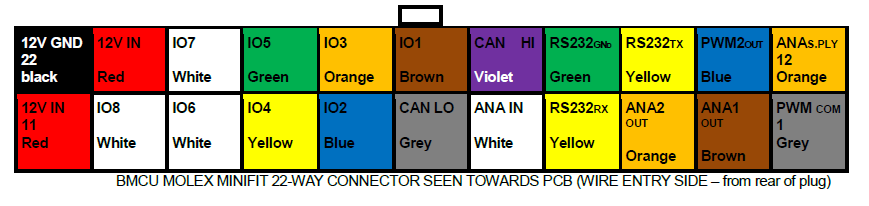
\includegraphics[width=0.9\linewidth]{Images/LithiumBalancePinout}}
		\caption{Brochage du connecteur Lithium Balance}
		\label{fig:lithiumbalancepinout}
	\end{figure}
	
	\begin{table}[H]
		\centering
		\caption{Nouveau brochage du connecteur de Lithium Balance}
		\label{22CLithiumBalance}	
		\begin{tabular}{ | l | l | l | l | }
			\hline
			Broche & Nom & Direction & Rôle \\ \hline
			1 & PWM COM & Sortie & Commun du signal de contrôle de la charge \\ \hline
			2 & ANA 1 OUT & Sortie & Signal analogique relié à la jauge de charge de la batterie \\ \hline
			3 & ANA 2 OUT & Entrée & Signal analogique pour contrôler le chargeur \\ \hline
			4 & RS232 RX & Entrée & Réception de la communication RS232 \\ \hline
			5 & ANA IN & Sortie & Non utilisé \\ \hline
			6 & CAN LO & Sortie & Niveau bas de la communication CAN \\ \hline
			7 & IO 2 & Sortie & Utilisé pour activer le pôle négatif du contacteur principal \\ \hline
			8 & IO 4 & Sortie & Utilisé pour la précharge du contacteur principal \\ \hline
			9 & IO 6 & Sortie & Sortie configurable par l'utilisateur \\ \hline
			10 & IO 8 & Sortie & Sortie configurable par l'utilisateur \\ \hline
			11 & 12V IN & Entrée & Alimentation 12V du système \\ \hline
			12 & ANA SUPPLY & Entrée & Alimentation externe de 0-30V pour le signal du chargeur \\ \hline
			13 & PWM 2 & Sortie & Modulation de largeur d'impulsion (PWM) pour le signal de charge \\ \hline
			14 & RS232 TX & Sortie & Transmission de la communication RS232 \\ \hline
			15 & RS232 GND & Sortie & Commun de la communication RS232 \\ \hline
			16 & CAN HI & Sortie & Niveau haut de la communication CAN \\ \hline
			17 & IO 1  & Sortie & Utilisé pour activer le pôle positif du contacteur principal \\ \hline
			18 & IO 3 & Entrée & Active le mode charge \\ \hline
			19 & IO 5 & Entrée & Active le mode décharge \\ \hline
			20 & IO 7 & Sortie & Sortie configurable par l'utilisateur \\ \hline
			21 & 12V IN & Entrée & Alimentation 12V du système \\ \hline
			22 & GND & Entrée & Commun du système \\ \hline
		\end{tabular}			
	\end{table}

	
	\subsubsection{Nouvelle configuration de brochage du connecteurs 22 pattes}	
		\paragraph*{}
		Certaines fonctions ont été ajoutées ou modifiés sans changer la compatibilité du connecteur. De plus, les broches pouvant être configurée par l'utilisateur ont de nouvelles fonctions. Par exemple, il y a une broche qui est utilisée pour la précharge du contacteurs MPPTs et trois alimentations de sortie tout-usages pour alimenter des ventilateurs ou autres appareils. Puis, les circuits analogiques sont inclus sur le module maître même s'il ne sont pas utilisés présentement par la voiture solaire. La nouvelle configuration du connecteurs 22 broches est détaillée par le tableau \ref{22CBmsEclipse}.
		
		\begin{table}[H]
			\centering
			\caption{Nouveau brochage du connecteur de Lithium Balance}
			\label{22CBmsEclipse}	
			
			\begin{tabular}{ | l | l | l | l | }
				\hline
				Broches & Nom & Direction & Rôle \\ \hline
				1 & PWM COM & Sortie & Commun du signal de contrôle de la charge \\ \hline
				2 & ANA 1 OUT & Sortie & Signal analogique tout usage \\ \hline
				3 & ANA 2 OUT & Entrée & Signal analogique tout usage \\ \hline
				4 & RS232 RX & Entrée & Réception de la communication RS232 \\ \hline
				5 & ANA IN & Sortie & Entrée analogique tout usage \\ \hline
				6 & CAN LO & Sortie & Niveau bas de la communication CAN \\ \hline
				7 & IO 2 & Sortie & Utilisé pour activer le pôle négatif du contacteur principal \\ \hline
				8 & IO 4 & Sortie & Utilisé pour la précharge du contacteur principal \\ \hline
				9 & IO 6 & Sortie & Utilisé pour la précharge du contacteur MPPT \\ \hline
				10 & IO 8 & Sortie & Alimentation de sortie tout usage \\ \hline
				11 & 12V IN & Entrée & Alimentation 12V du système \\ \hline
				12 & ANA SUPPLY & Entrée & Alimentation externe de 0-30V pour le signal du chargeur \\ \hline
				13 & PWM 2 & Sortie & Modulation de largeur d'impulsion (PWM) pour le signal de charge \\ \hline
				14 & RS232 TX & Sortie & Transmission de la communication RS232 \\ \hline
				15 & RS232 GND & Sortie & Commun de la communication RS232 \\ \hline
				16 & CAN HI & Sortie & Niveau haut de la communication CAN \\ \hline
				17 & IO 1  & Sortie & Utilisé pour activer le pôle négatif du contacteur principal \\ \hline
				18 & IO 3 & Entrée & Utilisé pour activer le contacteur des MPPTS \\ \hline
				19 & IO 5 & Entrée & Alimentation de sortie tout usage \\ \hline
				20 & IO 7 & Sortie & Alimentation de sortie tout usage \\ \hline
				21 & 12V IN & Entrée & Alimentation 12V du système \\ \hline
				22 & GND & Entrée & Commun du système \\ \hline
			\end{tabular}	
		\end{table}
